\section{Введение}

В данной работе исследуется принцип эквивалентности инертной и гравитационной масс. Проверка этого принципа проводится путем экспериментального измерения времени свободного падения тел из различных материалов, что позволяет подтвердить независимость ускорения свободного падения от массы и состава тела.

\subsection{Решаемые задачи}

\begin{enumerate}
    \item Проверить принцип эквивалентности масс.
    \item Измерить ускорения свободного падения тел.
    \item Познакомиться с методом измерения интервалов времени между импульсами частотомером — хронометром ЧЗ-32.
    \item Определить погрешность косвенных измерений.
\end{enumerate}

\section{Основная часть}

\subsection{Теоретическая часть}

\subsubsection{Равенство инертной и гравитационной масс}

Аристотель утверждал, что скорость падения тела зависит от его массы, но Галилей показал, что все тела падают с одинаковым ускорением в отсутствии сопротивления среды. Это привело к выводу о равенстве инертной и гравитационной масс.

Инертная масса определяется через ускорение под действием известной силы $|\vec{F}|$:
\begin{equation}
   M_{\text{ин}} = \frac{|\vec{F}|}{|\vec{a}|}
\end{equation}

Гравитационная масса определяется через силу тяготения:
\begin{equation}
   F = \gamma \frac{M_{\text{гр}} M_{\text{З}}}{r^2}
\end{equation}

\begin{equation}
   \quad M_{\text{гр}} = \frac{F r^2}{\gamma M_{\text{З}}}
\end{equation}

где $M_{\text{З}}$ — масса Земли, $\gamma$ — гравитационная постоянная, $r$ — расстояние между центром Земли и телом.

Докажем, что $M_{\text{гр}} = M_{\text{ин}}$. Для этого рассмотрим два тела с различными массами, падающие около поверхности Земли:
\begin{equation}
\label{eq:1}
   M^{(1)}_{\text{ин}}a_1 = \gamma \frac{M^{(1)}{\text{гр}}M_{\text{З}}}{R^2_{\text{З}}}
\end{equation}

\begin{equation}
\label{eq:2}
   M^{(2)}_{\text{ин}}a_2 = \gamma \frac{M^{(2)}_{\text{гр}}M_{\text{З}}}{R^2_{\text{З}}}
\end{equation}

Поделив уравнение (\ref{eq:1}) на уравнение (\ref{eq:2}), получаем:
\begin{equation}
   \frac{M_{\text{ин}}^{(1)}}{M_{\text{ин}}^{(2)}} \cdot\frac{a_1}{a_2} = \frac{M_{\text{гр}}^{(1)}}{M_{\text{гр}}^{(2)}}
\end{equation}

Из вывода Галилея известно, что $a_1 = a_2 = g$, поэтому:
\begin{equation}
\label{eq:3}
   \frac{M_{\text{ин}}^{(1)}}{M_{\text{гр}}^{(1)}} = \frac{M_{\text{ин}}^{(2)}}{M_{\text{гр}}^{(2)}} = const
\end{equation}

Соотношение работает для всех тел, экспериментально доказано, что $M_{\text{ин}} = M_{\text{гр}}$ с высокой точностью.

\subsubsection{Потенциальные поля и принцип эквивалентности}

Потенциальное поле — это поле, где работа по замкнутому контуру равна нулю:
\begin{equation}
\label{eq:4}
   A = \oint \vec{F} \cdot d\vec{l} = 0
\end{equation}

Принцип эквивалентности Эйнштейна утверждает, что в локальной системе отсчета, свободно падающей в гравитационном поле, законы физики совпадают с законами в инерциальной системе без гравитации. Уравнения движения в инерциальной системе:
\begin{equation}
\label{eq:5}
   m_k \frac{d^2\vec{x}_k}{dt^2} = m_k \vec{g} + \sum_{l \neq k} \vec{F}(\vec{x}_k - \vec{x}_l)
\end{equation}

После перехода в систему координат, движущуюся с ускорением $\vec{g}$:
\begin{equation}
\label{eq:6}
   \vec{x}\,' = \vec{x} - \frac{\vec{g}t^2}{2}, \quad t' = t
\end{equation}

Получаем:
\begin{equation}
\label{eq:7}
   m_k \frac{d^2\vec{x}_k'}{dt^2} = \sum_{l \neq k} \vec{F}(\vec{x}_k' - \vec{x}_l')
\end{equation}

Уравнение (\ref{eq:7}) совпадает с уравнением (\ref{eq:5}), если принять $\vec{g} = 0$. Таким образом, в достаточно малой области пространства-времени гравитационное поле можно компенсировать переходом в ускоренную систему отсчёта, делая законы физики локально идентичными их форме в отсутствие гравитации.

\subsection{Эксперимент}

Цель работы — проверить равенство времени свободного падения для тел разной массы.

На рис.~\ref{fig:photo} представлена фотография установки.

\begin{figure}[H]
\centering
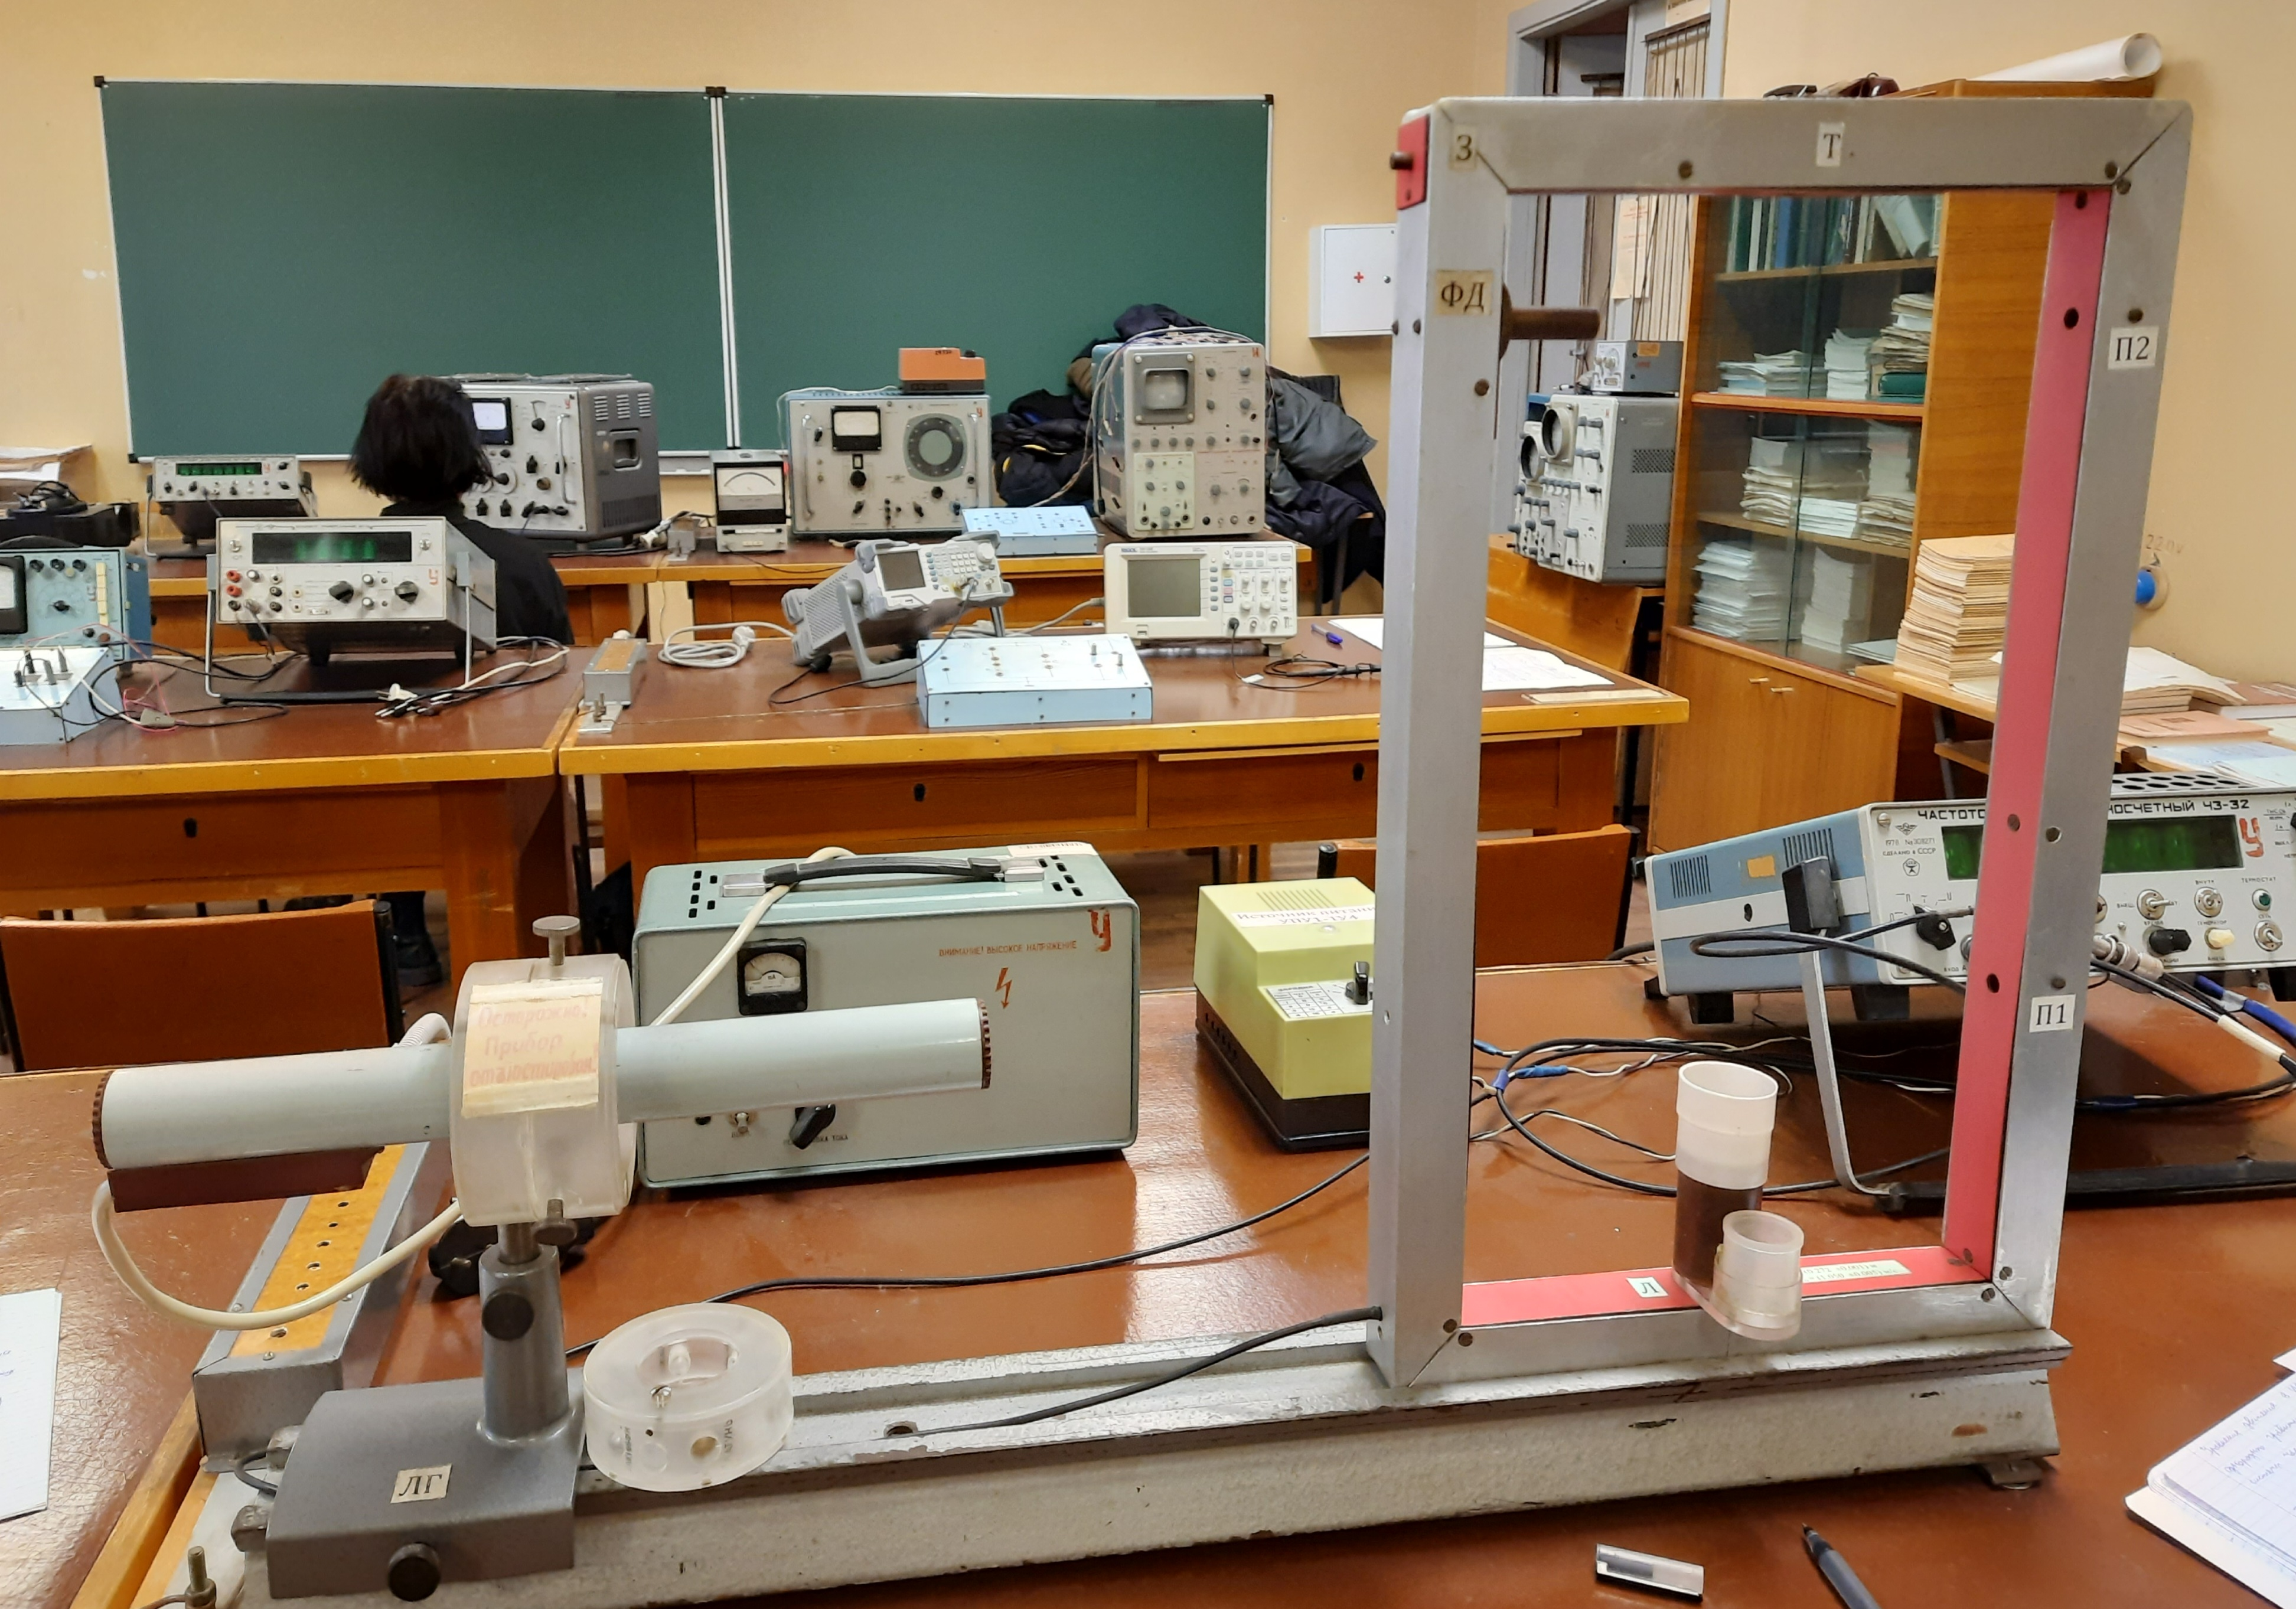
\includegraphics[width=0.8\textwidth]{photo.jpg}
\caption{Фотография установки}
\label{fig:photo}
\end{figure}

Схема установки представлена на рис.~\ref{fig:Scheme}. На схеме принимаются следующие обозначения:
\begin{itemize}
\item Т — трубка, в которой находится шарик.
\item З — заслонка, при отодвигании которой шарик должен упасть.
\item Л — луза, в которую должен упасть шарик.
\item ЛГ — луч квантового генератора, который дважды должен пересекаться шариком за время своего падения.
\item П$_1$, П$_2$ — призмы, отражающие луч генератора.
\item ФД — фотодиод, который вырабатывает импульс, усиливающийся в усилителе, при пересечении шариком луча генератора. От первого пересечения фотодиод импульсом запускает частотомер, отсчитывающий время падения шарика, а от второго — останавливает его.
\end{itemize}

\begin{figure}[H]
\centering
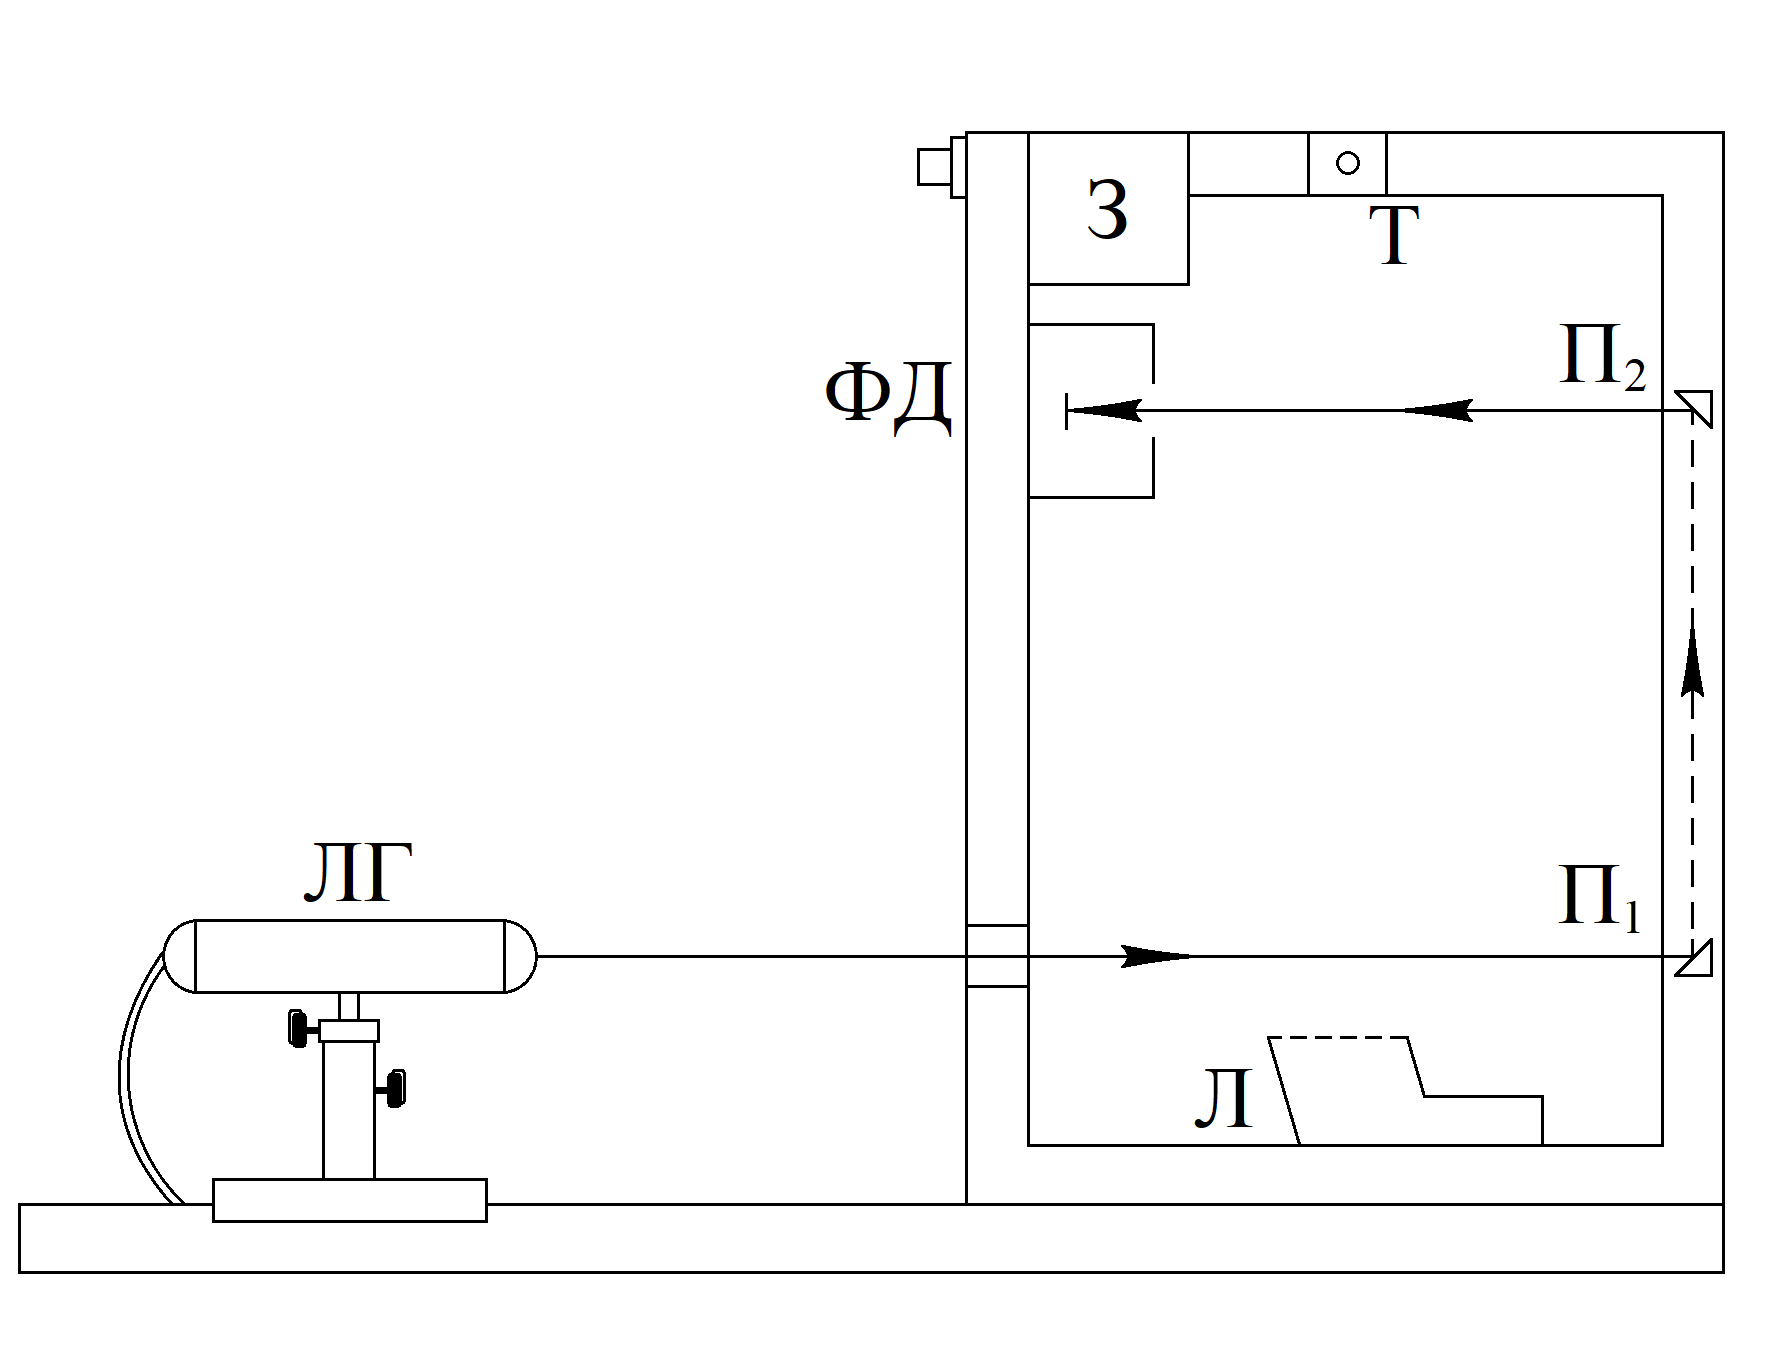
\includegraphics[width=0.9\textwidth]{Scheme.png}
\caption{Схема установки}
\label{fig:Scheme}
\end{figure}

Уравнение движения при свободном падении:
\begin{equation}
\label{eq:8}
   h = v_0 t + \frac{gt^2}{2}
\end{equation}

где $h$ — расстояние между лучами, $v_0$ — начальная скорость, а — $t$ время пролёта.
Из формулы (\ref{eq:8}) можно выразить ускорение свободного падения:
\begin{equation}
\label{eq:9}
   g = \frac{2(h - v_0 t)}{t^2}
\end{equation}

\subsection{Обработка данных и обсуждение результатов}
 
\subsubsection{Таблицы}

В ходе работы было проведено 180 измерений времени пролета шариков высоты $h = 0.272 \pm 0.001$ м по 30 измерений для каждого из шести материалов: алюминий, латунь, сталь, дерево, плексиглас, свинец. Известна $V_0 = 1.050 \pm 0.005$ м/с.

В таблице ~\ref{tabl:1} приведены плотности данных материалов, а также диаметры и массы шариков каждого материала, массы были высчитаны по формуле:
\begin{equation}
\label{eq:10}
   m = \rho \cdot V = \rho \cdot \left(\frac{4}{3} \pi r^3 \right)
\end{equation}

В таблице ~\ref{tabl:2} представлены экспериментально полученные данные измерений времени падения шариков, а также высчитаны их средние значения для каждого из материалов. В таблицах ~\ref{tabl:3}, ~\ref{tabl:4}, ~\ref{tabl:5} отражены результаты вычислений для шариков из тех же шести материалов погрешность $\Delta t$ времени падения шариков, ускорение свободного падения $g$ шариков и его погрешность $\Delta g$ соответственно.

\begin{center}
\begin{table}[H]
\centering
\caption{Параметры для различных материалов}
\label{tabl:1}
\renewcommand{\arraystretch}{1.15}
\begin{tabular}{|c|c|c|c|c|}
\hline
{} № п/п & Вещество & Плотность ($10^3$ кг/м$^3$) & Диаметр ($10^{-2}$ м) & Масса ($10^{-6}$ кг) \\
\hline
1 & Дерево     & 0,7   & 1 &  0.4 \\
2 & Плексиглас & 1,18  & 1 &  0.6 \\
3 & Алюминий   & 2,79  & 1 &  1   \\
4 & Сталь      & 7,9   & 1 &  4   \\
5 & Латунь     & 8,5   & 1 &  4   \\
6 & Свинец     & 11,34 & 1 &  6   \\
\hline
\end{tabular}
\end{table}
\end{center}

\begin{center}
\begin{table}[H]
\centering
\caption{Результаты измерения времени падения шарика}
\label{tabl:2}
\renewcommand{\arraystretch}{1.15}
\begin{tabular}{|c|c|c|c|c|c|c|}
\hline
{} & Алюминий & Латунь & Сталь & Дерево & Плексиглас & Свинец \\
\hline
{} № п.п. & t, мс & t, мс & t, мс & t, мс & t, мс & t, мс \\
\hline
1  & 153.711 & 153.039 & 152.657 & 154.106 & 153.791 & 153.170 \\
2  & 153.852 & 152.875 & 152.612 & 153.913 & 154.508 & 152.900 \\
3  & 153.329 & 154.192 & 152.649 & 154.585 & 153.987 & 153.384 \\
4  & 153.088 & 153.367 & 152.647 & 153.930 & 153.386 & 152.563 \\
5  & 153.404 & 153.577 & 152.680 & 153.995 & 153.998 & 152.203 \\
6  & 153.431 & 153.905 & 152.736 & 153.890 & 153.525 & 152.881 \\
7  & 154.129 & 153.155 & 152.590 & 153.983 & 154.117 & 153.407 \\
8  & 153.636 & 152.878 & 152.521 & 153.865 & 153.289 & 152.262 \\
9  & 153.469 & 153.254 & 152.759 & 153.927 & 153.557 & 153.524 \\
10 & 153.253 & 153.136 & 152.583 & 153.647 & 153.579 & 153.390 \\
11 & 153.364 & 153.136 & 152.836 & 154.282 & 153.798 & 153.742 \\
12 & 153.233 & 152.822 & 152.731 & 154.121 & 154.348 & 153.622 \\
13 & 153.798 & 153.004 & 152.647 & 153.838 & 153.567 & 153.585 \\
14 & 153.298 & 153.031 & 152.697 & 154.055 & 154.133 & 154.799 \\
15 & 154.312 & 152.896 & 152.595 & 154.854 & 154.271 & 153.538 \\
\hline
\end{tabular}
\end{table}
\end{center}







\begin{center}
\begin{table}[H]
\centering
\renewcommand{\arraystretch}{1.15}
\begin{tabular}{|c|c|c|c|c|c|c|}
\hline
16 & 153.805 & 153.338 & 152.695 & 154.219 & 154.379 & 153.299 \\
17 & 153.468 & 153.412 & 153.234 & 154.545 & 153.354 & 153.310 \\
18 & 153.242 & 153.154 & 152.861 & 154.266 & 153.508 & 153.925 \\
19 & 153.173 & 153.072 & 153.691 & 154.102 & 153.457 & 153.547 \\
20 & 153.624 & 152.948 & 153.219 & 154.126 & 153.844 & 153.877 \\
21 & 153.417 & 153.060 & 152.761 & 154.187 & 153.676 & 153.752 \\
22 & 152.930 & 152.905 & 152.742 & 154.580 & 153.427 & 154.052 \\
23 & 153.169 & 153.291 & 152.717 & 153.587 & 153.934 & 153.332 \\
24 & 153.379 & 153.032 & 152.891 & 155.155 & 153.348 & 153.924 \\
25 & 153.226 & 152.836 & 153.017 & 154.485 & 154.230 & 154.315 \\
26 & 153.202 & 153.059 & 152.957 & 153.993 & 153.658 & 153.865 \\
27 & 153.246 & 152.839 & 152.869 & 153.803 & 153.469 & 154.057 \\
28 & 152.514 & 152.999 & 152.854 & 154.108 & 153.975 & 153.459 \\
29 & 152.914 & 153.312 & 152.827 & 154.328 & 153.549 & 153.781 \\
30 & 153.729 & 153.089 & 152.797 & 153.985 & 153.444 & 154.085 \\
\hline
\begin{minipage}{2cm}
\begin{center}
    Среднее значение $\overline{t}$, с
\end{center}
\end{minipage}
& 153.412 & 153.154 & 152.802 & 154.149 & 153.770 & 153.518 \\
\hline
\end{tabular}
\end{table}
\end{center}

$\Delta t$ определяется как стандартная погрешность среднего значения по следующей формуле:
\begin{equation}
\label{eq:11}
   \Delta\overline{t}=\sqrt{\frac{\Sigma(t_i-\overline{t})^2}{{n(n-1)}}}
\end{equation}

\begin{center}
\begin{table}[H]
\centering
\caption{Погрешности $\Delta t$ времени пролета шариков}
\label{tabl:3}
\renewcommand{\arraystretch}{1.15}
\begin{tabular}{|c|c|}
\hline
\begin{minipage}{5cm}
\begin{center}
    Вещество 
\end{center}
\end{minipage} & 
\begin{minipage}{5cm}
\begin{center}
    $\Delta$t, мс 
\end{center}
\end{minipage} \\
\hline
Алюминий   & 0.0664068 \\
Латунь     & 0.0564740 \\
Сталь      & 0.0434949 \\
Дерево     & 0.0627690 \\
Плексиглас & 0.0643578 \\
Свинец     & 0.1030980 \\
\hline
\end{tabular}
\end{table}
\end{center}

Для таблицы ~\ref{tabl:4} были вычислены ускорения свободного падения для разных материалов по формуле (\ref{eq:8}).

\begin{center}
\begin{table}[H]
\centering
\caption{Ускорения свободного падения $g$ шариков}
\label{tabl:4}
\renewcommand{\arraystretch}{1.15}
\begin{tabular}{|c|c|}
\hline
\begin{minipage}{5cm}
\begin{center}
    Вещество 
\end{center}
\end{minipage} & 
\begin{minipage}{5cm}
\begin{center}
    $g$, м/с$^2$ 
\end{center}
\end{minipage} \\
\hline
Алюминий   & 9.43 \\
Латунь     & 9.48 \\
Сталь      & 9.56 \\
Дерево     & 9.27 \\
Плексиглас & 9.35 \\
Свинец     & 9.43 \\
\hline
\end{tabular}
\end{table}
\end{center}

Погрешность вычисляется как погрешность косвенных измерений по следующей формуле:

\begin{equation}
\label{eq:12}
   \Delta g = \sqrt{ \frac{1}{9} \left(\frac{\partial g}{\partial h}\right)^2 \Delta{h}^2 +
   \frac{1}{9} \left(\frac{\partial g}{\partial v_0}\right)^2 \Delta{v_0}^2 +
   \left(\frac{\partial g}{\partial t}\right)^2 \Delta{\overline{t}}^2}
\end{equation}

Пользуясь формулой (\ref{eq:9}) и вычисляя частные производные в формуле (\ref{eq:12}), получаем:

\begin{equation}
\label{eq:13}
   \Delta g = \sqrt{ \frac{1}{9} \left(\frac{2}{\overline{t}^2}\right)^2 \Delta{h}^2 +
   \frac{1}{9} \left(\frac{-2}{\overline{t}}\right)^2 \Delta{v_0}^2 +
   \left(\frac{2(v_0\overline{t}-2h)}{\overline{t}^3}\right)^2 \Delta{\overline{t}}^2}
\end{equation}

\begin{center}
\begin{table}[H]
\centering
\caption{Погрешности ускорения свободного падения $\Delta g$ шариков}
\label{tabl:5}
\renewcommand{\arraystretch}{1.15}
\begin{tabular}{|c|c|}
\hline
\begin{minipage}{5cm}
\begin{center}
    Вещество 
\end{center}
\end{minipage} & 
\begin{minipage}{5cm}
\begin{center}
    $\Delta g$, м/с$^2$ 
\end{center}
\end{minipage} \\
\hline
Алюминий   & 0.03 \\
Латунь     & 0.03 \\
Сталь      & 0.02 \\
Дерево     & 0.03 \\
Плексиглас & 0.03 \\
Свинец     & 0.03 \\
\hline
\end{tabular}
\end{table}
\end{center}

\subsubsection{Анализ возможных систематических погрешностей}

В ходе проведения эксперимента по измерению ускорения свободного падения могли возникнуть следующие систематические погрешности: связанные с установкой, погрешности измерения времени, погрешности от влияния внешних факторов.

Погрешности, связанные с установкой, могли возникнуть от неточности измерения высоты $h$, так как луч в ходе проведения лабораторной работы мог слегка отклониться, или за длительное время использования установки могли деформироваться отражающие призмы. Также для упрощения модели все шарики считались идеальными, однако они могли иметь небольшие отклонения от формы.

Погрешность измерения времени могла произойти из-за задержки импульса от фотодиода при пересечении луча генератора, а также от недостаточной точности измерения времени частотомером.

В качестве внешнего фактора могло выступить не учитываемое в данной работе сопротивление воздуха, тормозящее шарики при их падении, от чего измеряемое значение $g$ могло оказаться несколько меньше своего истинного значения.


\subsubsection{Описание программ}

Для обработки данных, связанных с измерением отношения заряда электрона к постоянной Больцмана, были разработаны две программы на языке C++. Эти программы предназначены для вычисления масс шариков из различных материалов и обработки экспериментальных данных времени падения шариков.

Программа ``mass\_calc'' на основе плотности и диаметра шариков из каждого материала вычисляет их массы, состоит из нескольких функций:
\begin{itemize}
\item in(): считывает данные из файла ``Input.csv'', где каждая строка содержит плотность материала (в $10^3$ кг/м$^3$) и диаметр шарика (в $10^{-2}$ м).
\item mass\_calc(): вычисляет массу шарика по формуле (\ref{eq:10}).
\item out(): записывает результаты в файл ``Output.csv'' с точностью до одного знака после запятой.
\end{itemize}

Программа ``calc\_values'' обрабатывает экспериментальные данные времени падения шариков и вычисляет погрешность времени $\overline{t}$, ускорение свободного падения $g$ и его погрешность $\Delta g$. Включает в себя следующие функции:

\begin{itemize}
\item in(): считывает данные из файла ``Input.csv'', содержащего время падения шариков для шести материалов (по 30 измерений для каждого).
\item tx(): вычисляет среднее время падения $\overline{t}$ для каждого материала.
\item gi(): рассчитывает ускорение свободного падения $g$ по формуле (\ref{eq:9}).
\item dt(): вычисляет погрешность времени $\Delta t$ как стандартную погрешность среднего значения по формуле (\ref{eq:11}).
\item dg(): Рассчитывает погрешность ускорения $\Delta g$ как погрешность косвенных измерений по следующей формуле (\ref{eq:13}).
\item out(): записывает результаты в файл ``Output.csv'', включая среднее время $\overline{t}$, его погрешность $\Delta t$, ускорение $g$ и его погрешность $\Delta g$.
\end{itemize}

\section{Вывод}
В ходе работы экспериментально подтверждён принцип эквивалентности масс: измеренные значения ускорения свободного падения для шариков разной массы и состава оказались равными в пределах погрешности ($g = 9.27 - 9.56$ м/с$^2$, $\Delta g = \pm 0.03$ м/с$^2$) Полученные результаты согласуются с теоретическими предсказаниями, демонстрируя независимость ускорения свободного падения от свойств падающего тела.

\begin{thebibliography}{9}
\bibitem{repo}
\url{https://github.com/st117208/Workshop4}  (дата обращения: 25.04.2025)
\end{thebibliography}